% Made up for the tikra gallery: a sine wave and the three numbers that shape it.
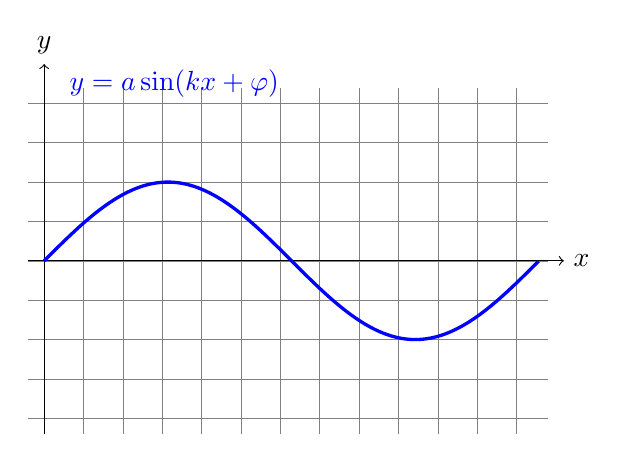
\begin{tikzpicture}
  \def\a{1}   % amplitude, 0..2
  \def\k{1}   % frequency, 0..4
  \def\p{0}   % phase in degrees, -180..180
  \draw[help lines, step=0.5] (-0.2,-2.2) grid (6.4,2.2);
  \draw[->] (-0.2,0) -- (6.6,0) node[right] {$x$};
  \draw[->] (0,-2.2) -- (0,2.5) node[above] {$y$};
  \draw[gray, dashed, domain=0:6.28, samples=100] plot (\x, {sin(deg(\x))});
  \draw[blue, very thick, domain=0:6.28, samples=160] plot (\x, {\a*sin(\k*deg(\x) + \p)});
  \node[blue, anchor=west] at (0.2,2.25) {$y = a\sin(kx + \varphi)$};
\end{tikzpicture}
